\documentclass[twoside,11pt]{homework}

\coursename{COMS W4705: Natural Language Processing (Fall 2018)} 

\studname{Wenbo Gao}    % YOUR NAME GOES HERE
\studmail{wg2313@columbia.edu}% YOUR UNI GOES HERE
\hwNo{2}                   % THE HOMEWORK NUMBER GOES HERE
\date{\today} % DATE GOES HERE

% Uncomment the next line if you want to use \includegraphics.
\usepackage{graphicx}
%\includegraphics[height=0.3\textheight]{hw0.pdf}
\usepackage{physics}
\usepackage{tikz}

\usetikzlibrary{fit,positioning,arrows,automata,calc}
\tikzset{
  main/.style={circle, minimum size = 15mm, thick, draw =black!80, node distance = 10mm},
  connect/.style={-latex, thick},
  box/.style={rectangle, minimum height = 8mm,draw=black!100}
}

% environments: theorem[*rename], proof[*rename], 

\begin{document}
\maketitle

\section*{Problem 1 - PCFGs and HHMs}
Both PCFGs and HMMs can be seen as generative models that produce a sequence of
POS tags and words with some probability (of course the PCFG will generate even
more structure, but it will also generate POS tags and words).

\subsection*{(a)}
\begin{prob}
  Revisit the example sentence "\textit{they are baking potatoes}" and grammar from
  Problem 2.
  For each sequence of POS tags that is possible for this sentence according to
  the grammar, what is the joint probability $P(\text{tags}, \text{words})$
  according to the PCFG?
  Hint: consider all parses for the sentence.
\end{prob}

\begin{solution}
  \ 

  first parse tree:\\
  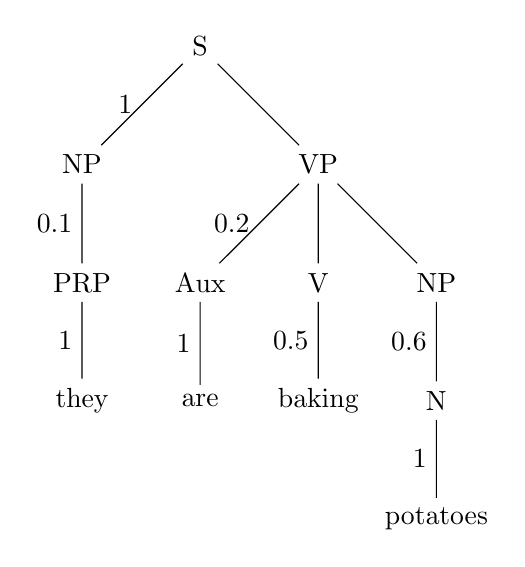
\begin{tikzpicture}
    [ level distance=1.5cm
    , level 1/.style={sibling distance=3cm}
    , level 2/.style={sibling distance=1.5cm}
    ]
  \node {S}
    child {node {NP}
      child {node {PRP}
        child {node {they}
          edge from parent {node[left] {1}}
        }
        edge from parent {node[left] {0.1}}
      }
      edge from parent {node[left] {1}}
    }
    child {node {VP}
      child {node {Aux}
        child {node {are}
          edge from parent {node[left] {1}}
        }
        edge from parent {node[left] {0.2}}
      }
      child {node {V}
        child {node {baking}
          edge from parent {node[left] {0.5}}
        }
      }
      child {node {NP}
        child {node {N}
          child {node {potatoes}
            edge from parent {node[left] {1}}
          }
          edge from parent {node[left] {0.6}}
        }
      }
    }
  ;
  \end{tikzpicture}

  There is only one possible parse tree (the first parse tree) given
  tags = \{PRP, Aux, V, N\},
  and words = \{they, are, baking, potatoes\}, thus
  \[
    \begin{aligned}
        &P[tags = \{PRP, Aux, V, N\}, words = \{they, are, baking, potatoes\}]\\
      = &\sum_{tree \in \{\text{parses tree with} \{they, are, baking, potatoes\} \text{as leaf nodes and} \{PRP, Aux, V, N\} \text{one layer above}\}} P[tree]\\
      = &P[\text{first parse tree}]\\
      = &0.006
    \end{aligned}
  \]

  second parse tree:\\
  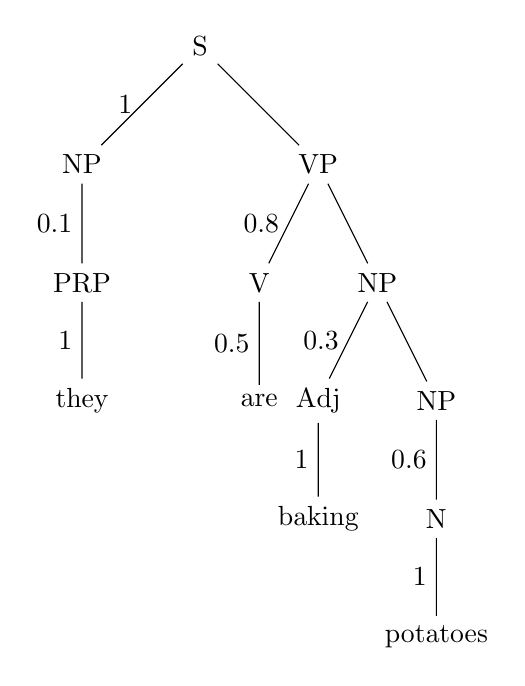
\begin{tikzpicture}
    [ level distance=1.5cm
    , level 1/.style={sibling distance=3cm}
    , level 2/.style={sibling distance=1.5cm}
    ]
  \node {S}
    child {node {NP}
      child {node {PRP}
        child {node {they}
          edge from parent {node[left] {1}}
        }
        edge from parent {node[left] {0.1}}
      }
      edge from parent {node[left] {1}}
    }
    child {node {VP}
      child {node {V}
        child {node {are}
          edge from parent {node[left] {0.5}}
        }
        edge from parent {node[left] {0.8}}
      }
      child {node {NP}
        child {node {Adj}
          child {node {baking}
            edge from parent {node[left] {1}}
          }
          edge from parent {node[left] {0.3}}
        }
        child {node {NP}
          child {node {N}
            child {node {potatoes}
              edge from parent {node[left] {1}}
            }
            edge from parent {node[left] {0.6}}
          }
        }
      }
    }
  ;
  \end{tikzpicture}

  There is only one possible parse tree given
  tags = \{ PRP, V, Adj, N\},
  and words = \{they, are, baking, potatoes\}, thus
  \[
    \begin{aligned}
        &P[tags = \{ PRP, V, Adj, N\}, words = \{they, are, baking, potatoes\}]\\
      = &\sum_{tree \in \{\text{parse trees with} \{they, are, baking, potatoes\} \text{as leaf nodes and} \{ PRP, V, Adj, N\} \text{one layer above}\}} P[tree]\\
      = &P[\text{second parse tree}]\\
      = &0.0072
    \end{aligned}
  \]
\end{solution}

\subsection*{(b)}

\begin{solution}
  \

  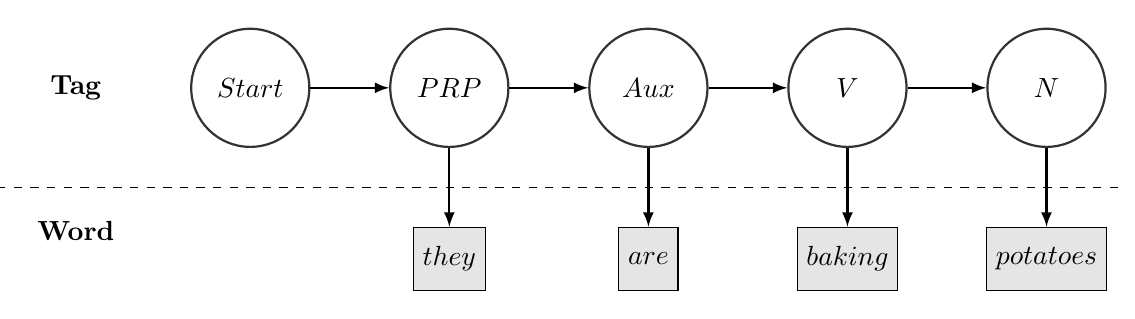
\begin{tikzpicture}
    \node[box,draw=white!100] (Latent) {\textbf{Tag}};
    \node[main] (Start) [right=of Latent] {$Start$};
    \node[main] (L1) [right=of Start] {$PRP$};
    \node[main] (L2) [right=of L1] {$Aux$};
    \node[main] (L3) [right=of L2] {$V$};
    \node[main] (Lt) [right=of L3] {$N$};
    \node[box,fill=black!10] (O1) [below=of L1] {$they$};
    \node[box,fill=black!10] (O2) [below=of L2] {$are$};
    \node[box,fill=black!10] (O3) [below=of L3] {$baking$};
    \node[box,fill=black!10] (Ot) [below=of Lt] {$potatoes$};
    \node[box,draw=white!100,below=of Latent] (Observed) {\textbf{Word}};

    \path (Start) edge [connect] (L1)
          (L1) edge [connect] (L2)
          (L2) edge [connect] (L3)
          (L3) edge [connect] (Lt);
    \path (L1) edge [connect] (O1)
          (L2) edge [connect] (O2)
          (L3) edge [connect] (O3)
          (Lt) edge [connect] (Ot);

    \draw [dashed, shorten >=-1cm, shorten <=-1cm]
        ($(Latent)!0.7!(Observed)$) coordinate (a) -- ($(Lt)!(a)!(Ot)$);
  \end{tikzpicture}

  \[
    \begin{aligned}
        &P[tags = \{PRP, Aux, V, N\}, words = \{they, are, baking, potatoes\}]\\
      = &P[tag = PRP | tag = Start] \cdot P[word = they | tag = PRP]\\
      \cdot &P[tag = Aux | tag = PRP] \cdot P[word = are | tag = Aux]\\
      \cdot &P[tag = V | tag = Aux] \cdot P[word = baking | tag = V]\\
      \cdot &P[tag = N | tag = V] \cdot P[word = potatoes | tag = N]\\
      = &0.006
    \end{aligned}
  \]

  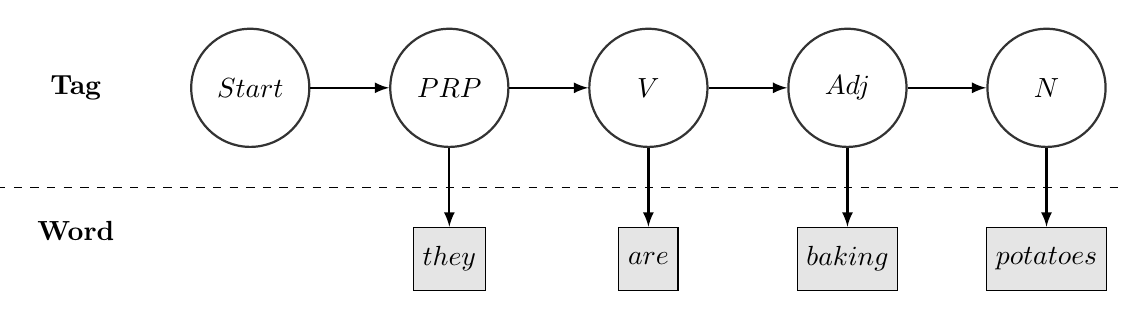
\begin{tikzpicture}
    \node[box,draw=white!100] (Latent) {\textbf{Tag}};
    \node[main] (Start) [right=of Latent] {$Start$};
    \node[main] (L1) [right=of Start] {$PRP$};
    \node[main] (L2) [right=of L1] {$V$};
    \node[main] (L3) [right=of L2] {$Adj$};
    \node[main] (Lt) [right=of L3] {$N$};
    \node[box,fill=black!10] (O1) [below=of L1] {$they$};
    \node[box,fill=black!10] (O2) [below=of L2] {$are$};
    \node[box,fill=black!10] (O3) [below=of L3] {$baking$};
    \node[box,fill=black!10] (Ot) [below=of Lt] {$potatoes$};
    \node[box,draw=white!100,below=of Latent] (Observed) {\textbf{Word}};

    \path (Start) edge [connect] (L1)
          (L1) edge [connect] (L2)
          (L2) edge [connect] (L3)
          (L3) edge [connect] (Lt);
    \path (L1) edge [connect] (O1)
          (L2) edge [connect] (O2)
          (L3) edge [connect] (O3)
          (Lt) edge [connect] (Ot);

    \draw [dashed, shorten >=-1cm, shorten <=-1cm]
        ($(Latent)!0.7!(Observed)$) coordinate (a) -- ($(Lt)!(a)!(Ot)$);
  \end{tikzpicture}
  \[
    \begin{aligned}
        &P[tags = \{PRP, V, Adj, N\}, words = \{they, are, baking, potatoes\}]\\
      = &P[tag = PRP | tag = Start] \cdot P[word = they | tag = PRP]\\
      \cdot &P[tag = V | tag = PRP] \cdot P[word = are | tag = V]\\
      \cdot &P[tag = Adj | tag = V] \cdot P[word = baking | tag = Adj]\\
      \cdot &P[tag = N | tag = Adj] \cdot P[word = potatoes | tag = N]\\
      = &0.0072
    \end{aligned}
  \]

  Here is my HMM:
  \begin{enumerate}
  \item tag-word transition distributions (the same as in PCFG):
    \begin{itemize}
    \item $P[word = they | tag = PRP] = 1$
    \item $P[word = are | tag = Aux] = 1$
    \item $P[word = baking | tag = V] = 0.5$, $P[word = are | tag = V] = 0.5$
    \item $P[word = potatoes | tag = N] = 1$
    \end{itemize}
  \item tag-tag transition distributions:
    \begin{itemize}
    \item $P[tag = PRP | tag = Start] = 1$
    \item $P[tag = Aux | tag = PRP] = 0.5$, $P[tag = V | tag = PRP] = 0.5$
    \item $P[tag = N | tag = V] = 0.5$, $P[tag = Adj | tag = V] = 0.5$
    \item $P[tag = V | tag = Aux] = 0.048$, $P[tag = PRP | tag = Aux] = 0.952$
    \item $P[tag = N | tag = Adj] = 0.0576$
    \item $P[tag = PRP | tag = N] = 1$
    \end{itemize}
  \end{enumerate}

\end{solution}

\subsection*{(c)}
\begin{prob}
  In general, is it possible to translate any PCFG into an HMM that produces the
  identical \textit{joint} probability P(tags, words) as PCFG (i.e. not just for
  a single sentence)? Explain how or why not. No formal proof is necessary.
  Hint: This has nothing to do with probabilities, but with language classes.
\end{prob}
\begin{solution}
  The hidden/latent state space in HMM can be formally described
  by a finite state machine which is strictly less expressive than pushdown
  automaton / context-free grammar in PCFG.
\end{solution}

\section*{Problem 2}

Consider the following probabilistic context free grammar.

\[
  \begin{aligned}
    S &\rightarrow NP\ VP &[1.0]\\
    NP &\rightarrow Adj\ NP &[0.3]\\
    NP &\rightarrow PRP &[0.1]\\
    NP &\rightarrow N &[0.6]\\
    VP &\rightarrow V\ NP &[0.8]\\
    VP &\rightarrow Aux\ V\ NP &[0.2]\\
    PRP &\rightarrow they &[1.0]\\
    N &\rightarrow potatoes &[1.0]\\
    Adj &\rightarrow baking &[1.0]\\
    V &\rightarrow baking &[0.5]\\
    V &\rightarrow are &[0.5]\\
    Aux &\rightarrow are &[1.0]\\
  \end{aligned}
\]

\subsection*{(a)}
\begin{prob}
  Using this grammar, show how the \textbf{Earley algorithm} would parse the
  following sentence.

  \textit{they are baking potatoes}

  Write down the complete parse chart.
  The chart should contain $n + 1$ entries where $n$ is the length of the
  sentence.
  Each entry $i$ should contain \textit{all} parser items generated by the
  parser that end in position $i$.
  You can ignore the probability for part (a).
\end{prob}

\begin{solution}
  \

  \textbf{Chart[0]} \\
  $>$ init\\
  $s0$: S $\rightarrow \cdot$ NP VP [0,0]\\
  $>$ predict $s0$, $_0|$NP$|_1$\\
  $s1$: NP $\rightarrow \cdot$ Adj NP [0,0]\\
  $s2$: NP $\rightarrow \cdot$ PRP [0,0]\\
  $s3$: NP $\rightarrow \cdot$ N [0,0]\\
  $>$ predict $s1$, $_0|$Adj$|_1$\\
  $s4$: Adj $\rightarrow \cdot$ baking [0,0]\\
  $>$ predict $s2$, $_0|$PRP$|_1$\\
  $s5$: PRP $\rightarrow \cdot$ they [0,0]\\
  $>$ predict $s3$, $_0|$N$|_1$\\
  $s6$: N $\rightarrow \cdot$ potatoes [0,0]\\
  $>$ scan $s4$, $_0|$baking$|_1$, failure\\
  $>$ scan $s5$, $_0|$they$|_1$, success\\

  \textbf{Chart[1]}\\
  $s7$: PRP $\rightarrow$ they$\cdot$ [0,1]\\
  $>$ scan $s6$, $_0|$potatoes$|_1$, failure\\
  $>$ complete with $s7$, $_0|$PRP$|_1$, traverse Chart[0]\\
  $.$ hit $s2$\\
  $s8$: NP $\rightarrow$ PRP $\cdot$ [0,1]\\
  $>$ complete with $s8$, $_0|$NP$|_1$, traverse Chart[0]\\
  $.$ hit $s0$\\
  $s9$: S $\rightarrow$ NP $\cdot$ VP [0,1]\\
  $>$ predict $s9$, $_1|$VP$|_2$\\
  $s10$: VP $\rightarrow \cdot$ V NP [1,1]\\
  $s11$: VP $\rightarrow \cdot$ Aux V NP [1,1]\\
  $>$ predict $s10$, $_1|$V$|_2$\\
  $s12$: V $\rightarrow \cdot$ baking [1,1]\\
  $s13$: V $\rightarrow \cdot$ are [1,1]\\
  $>$ predict $s11$, $_1|$Aux$|_2$\\
  $s14$: Aux $\rightarrow \cdot$ are [1,1]\\
  $>$ scan $s12$, $_1|$baking$|_2$, failure\\
  $>$ scan $s13$, $_1|$are$|_2$, success\\

  \textbf{Chart[2]}\\
  $s15$: V $\rightarrow$ are $\cdot$ [1,2]\\
  $>$ scan $s14$, $_1|$are$|_2$, success\\
  $s16$: Aux $\rightarrow$ are $\cdot$ [1,2]\\
  $>$ complete with $s15$, $_1|$V$|_2$, traverse Chart[1]\\
  $.$ hit $s10$\\
  $s17$: VP $\rightarrow$ V $\cdot$ NP [1,2]\\
  $>$ complete with $s16$, $_1|$Aux$|_2$, traverse Chart[1]\\
  $.$ hit $s11$\\
  $s18$: VP $\rightarrow$ Aux $\cdot$ V NP [1,2]\\
  $>$ predict $s17$, $_2|$NP$|_3$\\
  $s19$: NP $\rightarrow \cdot$Adj NP [2,2]\\
  $s20$: NP $\rightarrow \cdot$PRP [2,2]\\
  $s21$: NP $\rightarrow \cdot$N [2,2]\\
  $>$ predict $s18$, $_2|$V$|_3$\\
  $s22$: V $\rightarrow \cdot$ baking [2,2]\\
  $s23$: V $\rightarrow \cdot$ are [2,2]\\
  $>$ predict $s19$, $_2|$Adj$|_3$\\
  $s24$: Adj $\rightarrow \cdot$ baking [2,2]\\
  $>$ predict $s20$, $_2|$PRP$|_3$\\
  $s25$: PRP $\rightarrow \cdot$ they [2,2]\\
  $>$ predict $s21$, $_2|$N$|_3$\\
  $s26$: N $\rightarrow \cdot$ potatoes [2,2]\\
  $>$ scan $s22$, $_2|$baking$|_3$, success\\

  \textbf{Chart[3]}\\
  $s27$: V $\rightarrow$ baking $\cdot$ [2,3]\\
  $>$ scan $s23$, $_2|$are$|_3$, failure\\
  $>$ scan $s24$, $_2|$baking$|_3$, success\\
  $s28$: Adj $\rightarrow$ baking $\cdot$ [2,3]\\
  $>$ scan $s25$, $_2|$they$|_3$, failure\\
  $>$ scan $s26$, $_2|$potatoes$|_3$, failure\\
  $>$ complete with $s27$, $_2|$V$|_3$, traverse Chart[2]\\
  $.$ hit $s18$\\
  $s29$: VP $\rightarrow$ Aux V $\cdot$ NP [1,3]\\
  $>$ complete with $s28$, $_2|$Adj$|_3$, traverse Chart[3]\\
  $.$ hit $s19$\\
  $s30$: NP $\rightarrow$ Adj $\cdot$ NP [2,3]\\
  $>$ predict $s29$, $_3|$NP$|_4$\\
  $s31$: NP $\rightarrow \cdot$ Adj NP [3,3]\\
  $s32$: NP $\rightarrow \cdot$ PRP [3,3]\\
  $s33$: NP $\rightarrow \cdot$ N [3,3]\\
  $>$ predict $s30$, $_3|$NP$|_4$, duplicate\\
  $>$ predict $s31$, $_3|$Adj$|_4$\\
  $s34$: Adj $\rightarrow \cdot$ baking [3,3]\\
  $>$ predict $s32$, $_3|$PRP$|_4$\\
  $s35$: PRP $\rightarrow \cdot$ they [3,3]\\
  $>$ predict $s33$, $_3|$N$|_4$\\
  $s36$: N $\rightarrow \cdot$ potatoes [3,3]\\
  $>$ scan $s34$, $_3|$baking$|_4$, failure\\
  $>$ scan $s35$, $_3|$they$|_4$, failure\\
  $>$ scan $s36$, $_3|$potatoes$|_4$, success\\

  \textbf{Chart[4]}\\
  $s37$: N $\rightarrow$ potatoes $\cdot$ [3,4]\\
  $>$ complete with $s37$, $_3|$N$|_4$, traverse Chart[3]\\
  $.$ hit $s33$\\
  $s38$: NP $\rightarrow$ N $\cdot$ [3,4]\\
  $>$ complete with $s38$, $_3|$NP$|_4$, traverse Chart[3]\\
  $.$ hit $s29$\\
  $s39$: VP $\rightarrow$ Aux V NP $\cdot$ [1,4]\\
  $.$ hit $s30$\\
  $s40$: NP $\rightarrow$ Adj NP $\cdot$ [2,4]\\
  $>$ complete with $s39$, $_1|$VP$|_4$, traverse Chart[1]\\
  $.$ hit $s9$\\
  $s41$: S $\rightarrow$ NP VP $\cdot$ [0,4], \textbf{solution 1}($s9$, $s39$)\\
  $>$ complete with $s40$, $_2|$NP$|_4$, traverse Chart[2]\\
  $.$ hit $s17$\\
  $s42$: VP $\rightarrow$ V NP $\cdot$ [1,4]\\
  $>$ complete with $s42$, $_1|$VP$|_4$, traverse Chart[1]\\
  $.$ hit $s9$\\
  S $\rightarrow$ NP VP $\cdot$ [0,4], duplicate of $s41$, \textbf{solution 2}($s9$, $s42$)\\
  
\end{solution}

\subsection*{(b)}
\begin{prob}
  Write down \textit{all} parse trees for the sentence and grammar from problem
  2 and compute their probabilities according to the PCFG.
\end{prob}

\begin{solution}

  first parse tree:\\
  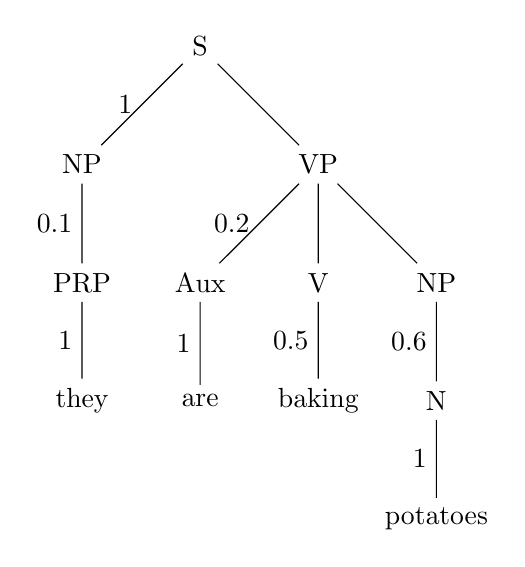
\begin{tikzpicture}
    [ level distance=1.5cm
    , level 1/.style={sibling distance=3cm}
    , level 2/.style={sibling distance=1.5cm}
    ]
  \node {S}
    child {node {NP}
      child {node {PRP}
        child {node {they}
          edge from parent {node[left] {1}}
        }
        edge from parent {node[left] {0.1}}
      }
      edge from parent {node[left] {1}}
    }
    child {node {VP}
      child {node {Aux}
        child {node {are}
          edge from parent {node[left] {1}}
        }
        edge from parent {node[left] {0.2}}
      }
      child {node {V}
        child {node {baking}
          edge from parent {node[left] {0.5}}
        }
      }
      child {node {NP}
        child {node {N}
          child {node {potatoes}
            edge from parent {node[left] {1}}
          }
          edge from parent {node[left] {0.6}}
        }
      }
    }
  ;
  \end{tikzpicture}

  \[
    \begin{aligned}
        &P[\text{first parse tree}]\\
      = &P[S \rightarrow NP\ VP] \cdot P[NP \rightarrow PRP] \cdot P[VP \rightarrow Aux\ V\ NP] \cdot P[PRP \rightarrow they]\\
        &\cdot P[Aux \rightarrow are] \cdot P[V \rightarrow baking] \cdot P[NP \rightarrow N] \cdot P[N \rightarrow potatoes]\\
      = &1 \cdot 0.1 \cdot 0.2 \cdot 1 \cdot 1 \cdot 0.5 \cdot 0.6 \cdot 1\\
      = &0.006
    \end{aligned}
  \]

  second parse tree:\\
  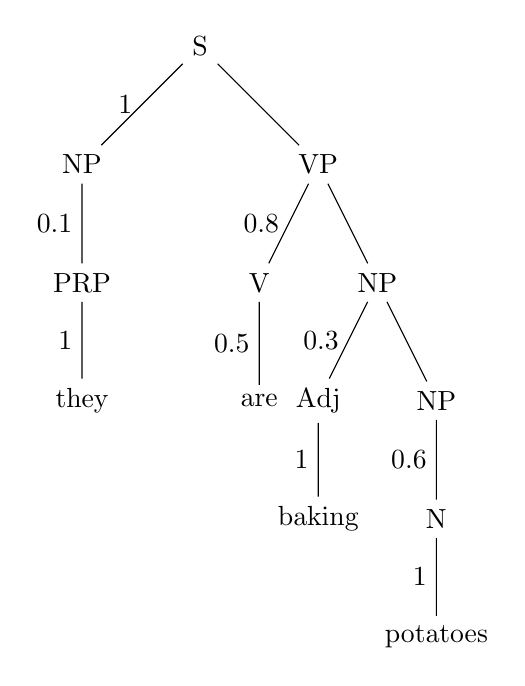
\begin{tikzpicture}
    [ level distance=1.5cm
    , level 1/.style={sibling distance=3cm}
    , level 2/.style={sibling distance=1.5cm}
    ]
  \node {S}
    child {node {NP}
      child {node {PRP}
        child {node {they}
          edge from parent {node[left] {1}}
        }
        edge from parent {node[left] {0.1}}
      }
      edge from parent {node[left] {1}}
    }
    child {node {VP}
      child {node {V}
        child {node {are}
          edge from parent {node[left] {0.5}}
        }
        edge from parent {node[left] {0.8}}
      }
      child {node {NP}
        child {node {Adj}
          child {node {baking}
            edge from parent {node[left] {1}}
          }
          edge from parent {node[left] {0.3}}
        }
        child {node {NP}
          child {node {N}
            child {node {potatoes}
              edge from parent {node[left] {1}}
            }
            edge from parent {node[left] {0.6}}
          }
        }
      }
    }
  ;
  \end{tikzpicture}

  \[
    \begin{aligned}
        &P[\text{second parse tree}]\\
      = &P[S \rightarrow NP\ VP] \cdot P[NP \rightarrow PRP] \cdot P[VP \rightarrow V\ NP] \cdot P[PRP \rightarrow they]\\
        &\cdot P[V \rightarrow are] \cdot P[NP \rightarrow Adj\ NP] \cdot P[Adj \rightarrow baking] \cdot P[NP \rightarrow N] \cdot P[N \rightarrow potatoes]\\
      = &1 \cdot 0.1 \cdot 0.8 \cdot 1 \cdot 0.5 \cdot 0.3 \cdot 1 \cdot 0.6 \cdot 1\\
      = &0.0072
    \end{aligned}
  \]

\end{solution}

\section*{Problem 3 - CKY parsing}
\subsection*{(a)}

\begin{prob}
  Convert the grammar from problem 2 into an equivalent grammra in Chomsky
  Normal Form (CNF).
  Write down the new grammar.
  Also explain what the general rule is for dealing with
  \begin{enumerate}
  \item Rules of the form A $\rightarrow$ B (i.e. a single non-terminal no the right hand side).
  \item Rules with three or more non-terminals on the right hand side (e.g. A $\rightarrow$
    B C D E).
  \end{enumerate}

  You don not have to deal with the case in which terminals and non-terminals
  are mixed in a rule right-hand side.
  You also do not have to convert the probabilites.
  Hint: Think about adding new non-terminal symbols.
\end{prob}

\begin{solution}
  \

  New grammar:
  \[
    \begin{aligned}
      \text{S} &\rightarrow \text{NP VP} &[0.3]\\
      \text{S} &\rightarrow \text{PRP VP} &[0.1]\\
      \text{S} &\rightarrow \text{N VP} &[0.6]\\
      \hline
      \text{NP} &\rightarrow \text{Adj NP} &[0.3]\\
      \text{NP} &\rightarrow \text{Adj PRP} &[0.1]\\
      \text{NP} &\rightarrow \text{Adj N} &[0.6]\\
      \hline
      \text{VP} &\rightarrow \text{V NP} &[0.24]\\
      \text{VP} &\rightarrow \text{V PRP} &[0.08]\\
      \text{VP} &\rightarrow \text{V N} &[0.48]\\
      \text{VP} &\rightarrow \text{AV NP} &[0.06]\\
      \text{VP} &\rightarrow \text{AV PRP} &[0.02]\\
      \text{VP} &\rightarrow \text{AV N} &[0.12]\\
      \hline
      \text{AV} &\rightarrow \text{Aux V} &[1.0]\\
    \end{aligned}
  \]

  General rules:
  \begin{enumerate}
  \item for A $\rightarrow$ B
    \begin{itemize}
    \item find all rules with A on the right-hand side, e.g. C $\rightarrow$ A D
    \item for each of them, substitute A on the right-hand side by B,
      i.e. C $\rightarrow$ B D
    \item add the modified rules to the rule set, and remove the original rule
    \end{itemize}
  \item for A $\rightarrow$ B C D E
    \begin{itemize}
    \item add non-terminals \{ F, G \}
    \item add rules:
      \begin{enumerate}
      \item A $\rightarrow$ B F
      \item F $\rightarrow$ C G
      \item G $\rightarrow$ D E
      \end{enumerate}
    \item remove the original rule
    \end{itemize}
  \end{enumerate}
\end{solution}

\subsection*{(b)}
\begin{prob}
  Using your grammar, fill the CKY parse chart as shown in class and show all
  parse trees.
\end{prob}

\begin{solution}
  See Figure \ref{fig:01}.
  \begin{figure}[h]
  	\centering
  	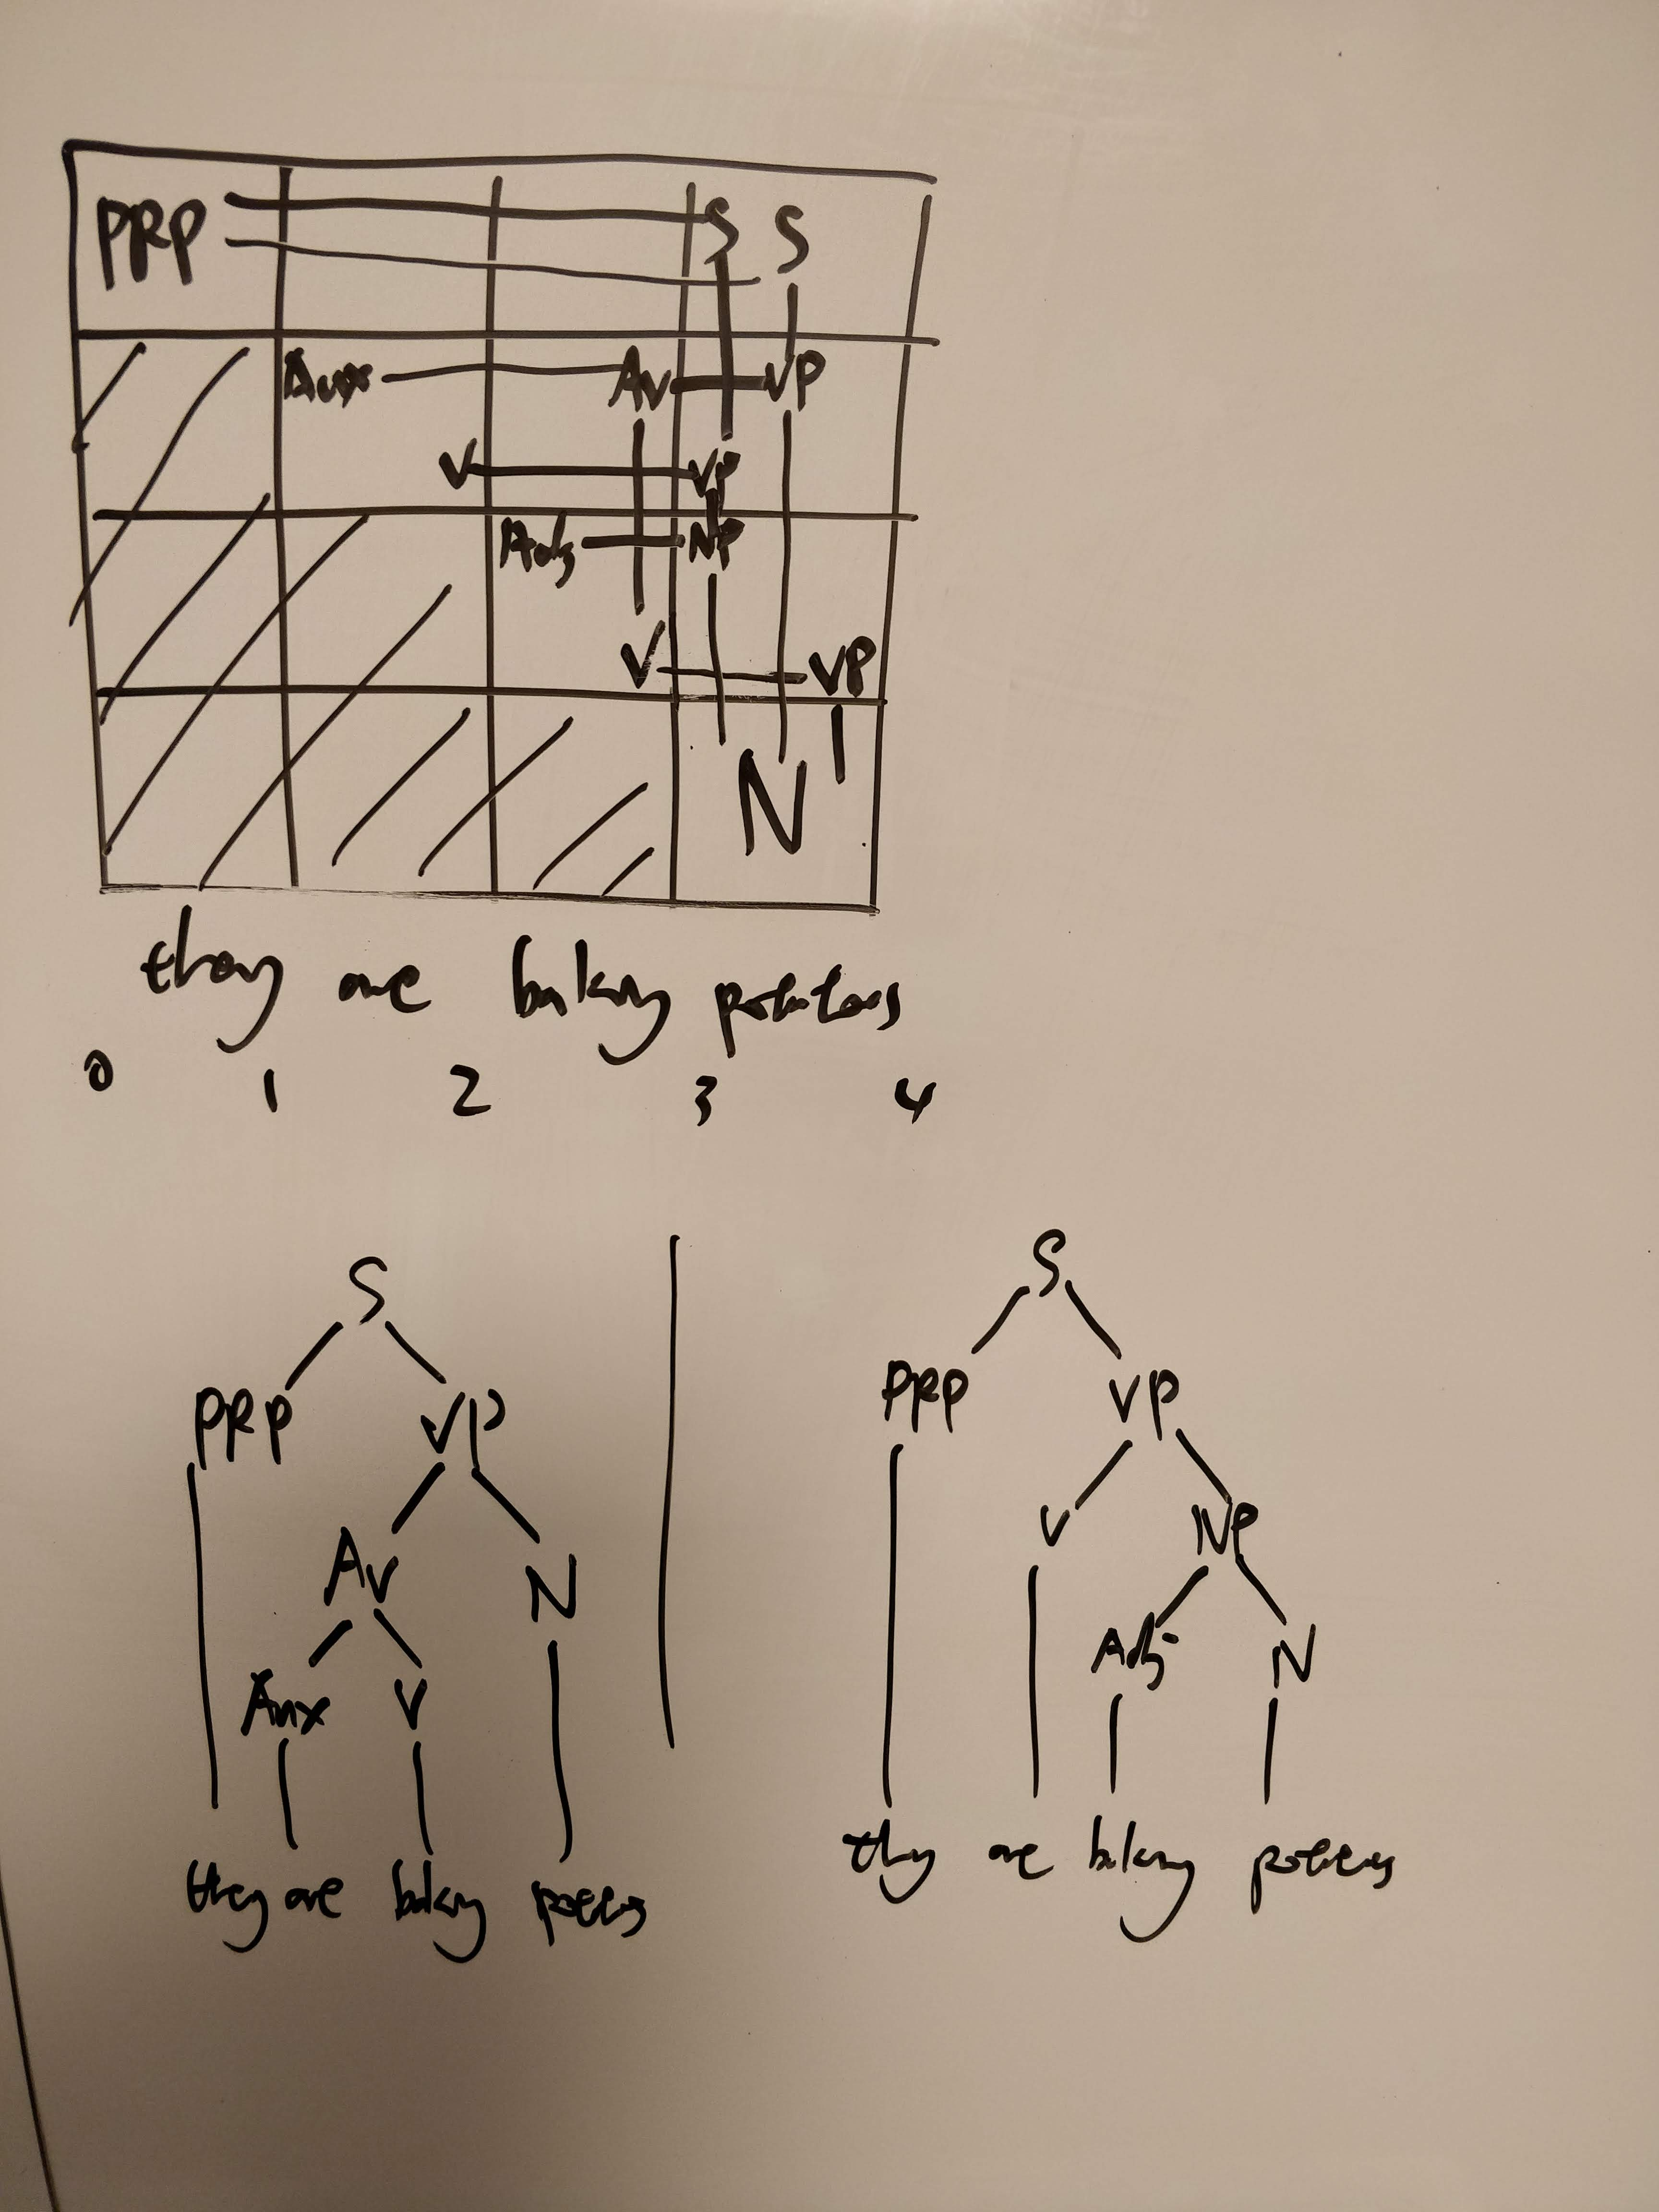
\includegraphics[width=0.7\linewidth]{../03-2}
  	\caption{problem 3 (b)}
  	\label{fig:01}
  \end{figure}
  
\end{solution}

\section*{Problem 4 - Transition Based Dependency Parsing}
\begin{prob}
  Consider the following dependency graph.
    \begin{figure}[h]
      \centering
      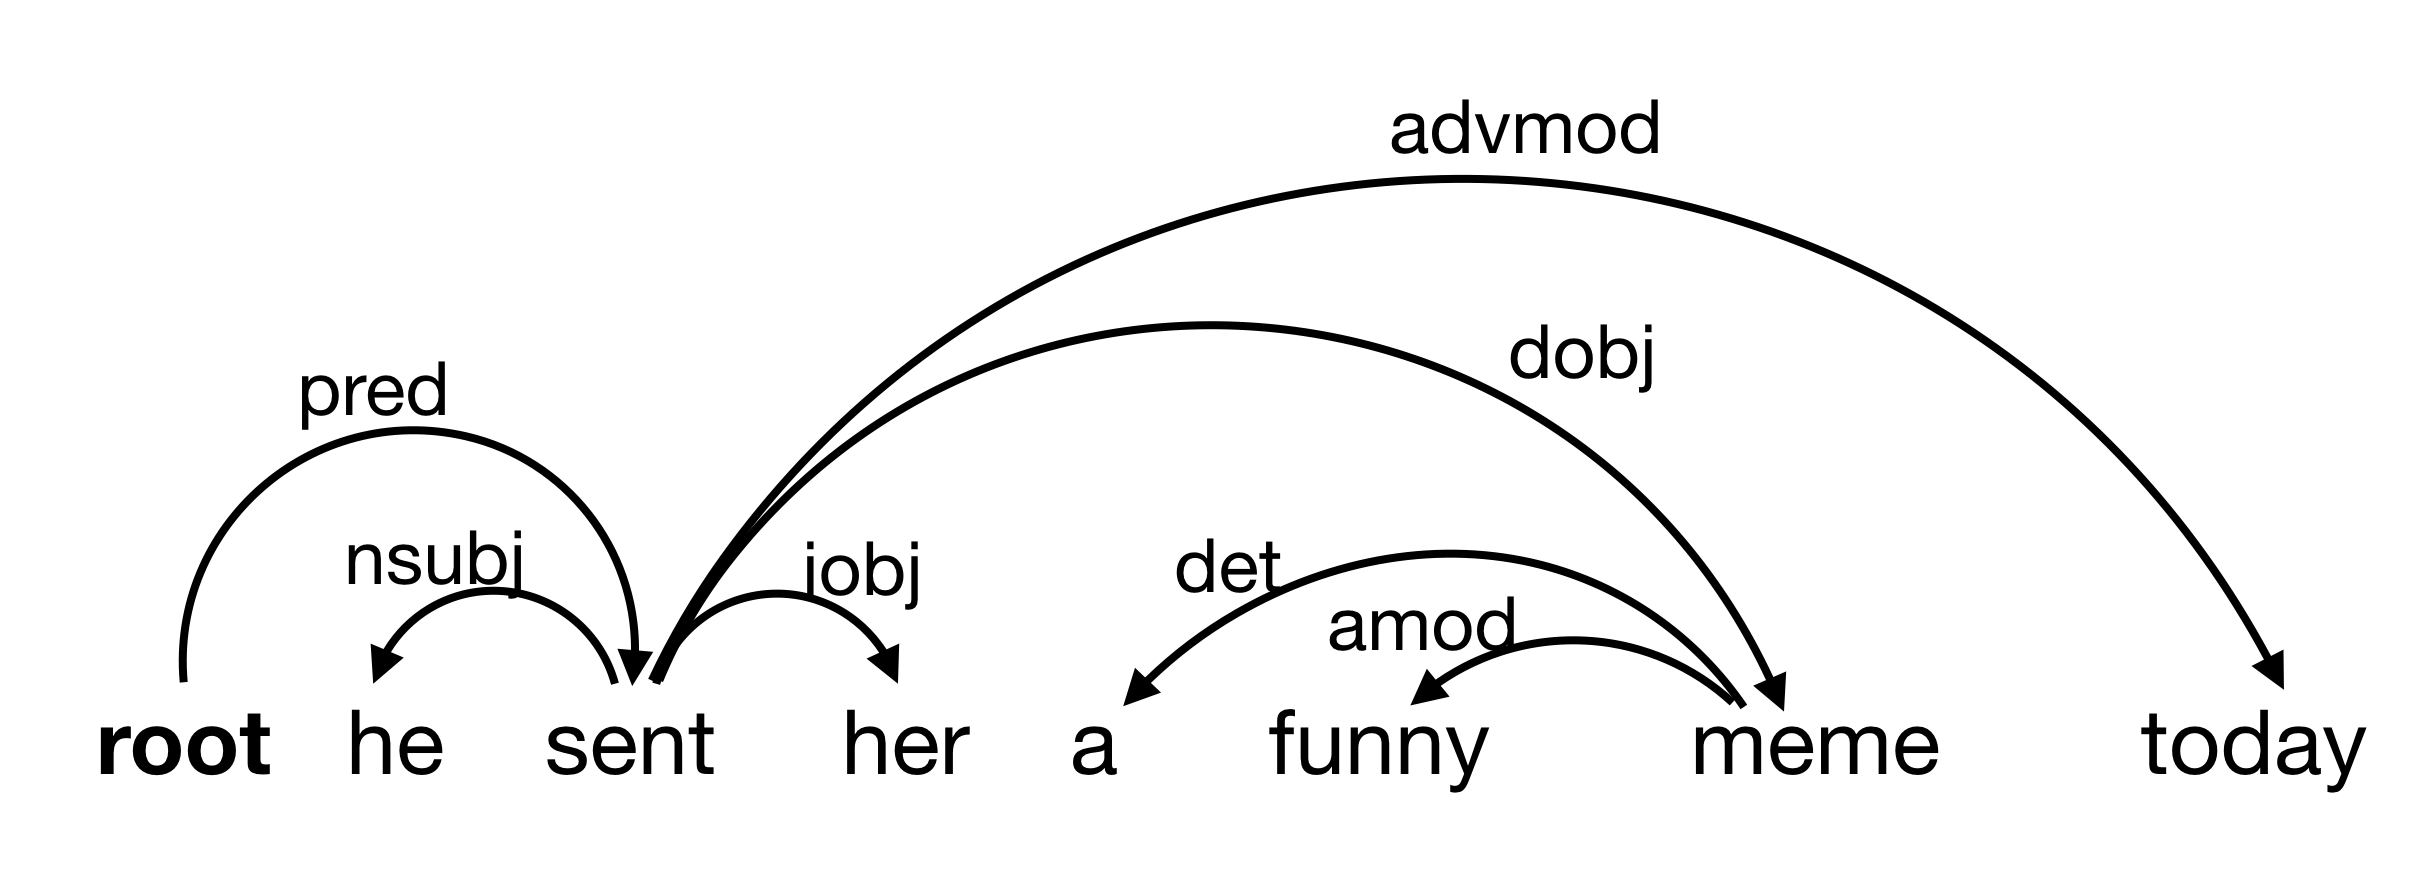
\includegraphics[width=0.7\linewidth]{../materials/he_sent_her_a_funny_meme_today}
      \label{fig:02}
    \end{figure}
  Write down the sequence of transitions that an arc-standard dependency parser
  would have to take to generate this dependency tree from the initial state.

  ([\textbf{root}]$\sigma$, [he, sent, her, a, funny, meme, today]$\beta$, \{\}A)

  Also write down the state resulting from each transition.
\end{prob}

\begin{solution}
  \ \\
  s0: [root], [he, send, her, a, funny, meme, today], []\\
  $>$ shift\\
  s1: [root, he], [send, her, a, funny, meme, today], []\\
  $>$ Left-Arc$_{\text{nsubj}}$\\
  s2: [root], [send, her, a, funny, meme, today], [(send, nsubj, he)]\\
  $>$ shift\\
  s3: [root, send], [her, a, funny, meme, today], [...]\\
  $>$ Right-Arc$_{\text{jobj}}$\\
  s4: [root], [send, a, funny, meme, today], [..., (send, jobj, her)]\\
  $>$ shift\\
  s5: [root, send], [a, funny, meme, today], [...]\\
  $>$ shift\\
  s6: [root, send, a], [funny, meme, today], [...]\\
  $>$ shift\\
  s7: [root, send, a, funny], [meme, today], [...]\\
  $>$ Left-Arc$_{\text{amod}}$\\
  s8: [root, send, a], [meme, today], [..., (meme, amod, funny)]\\
  $>$ Left-Arc$_{\text{det}}$\\
  s9: [root, send], [meme, today], [..., (meme, det, a)]\\
  $>$ Right-Arc$_{\text{dobj}}$\\
  s10: [root], [send, today], [..., (send, dobj, meme)]\\
  $>$ shift\\
  s11: [root, send], [today], [...]\\
  $>$ Right-Arc$_{\text{advmod}}$\\
  s12: [root], [send], [..., (send, advmod, today)]\\
  $>$ Right-Arc$_{\text{pred}}$\\
  s13: [], [root], [..., (root, pred, send)]\\
  $>$ shift\\
  s14: [root], [], [...]\\
  
\end{solution}


\end{document} 
